%-------------------------------------------------------------------------
%  paper.tex -- The basic outline of the paper, includes all the sections
%
%   $Id$
%-------------------------------------------------------------------------


\documentclass{article}
\usepackage{fullpage}
%\usepackage{fancybox}
\usepackage{graphicx}
\usepackage{rotating}
\usepackage{lscape}
\usepackage{personal}

\newcommand{\pcp}{\mbox{\textsf{PCp}$^3$}}
\newcommand{\pcppp}{\mbox{\textsf{PCppP}}}
\newcommand{\Cpp}{\mbox{\textsf{cpp}}}
\newcommand{\CPP}{\mbox{\textsf{C++}}}
\newcommand{\Perl}{\mbox{\textsf{Perl}}}
\newcommand{\C}{\mbox{\textsf{C}}}

\newcommand{\backcall}[3]{\item \texttt{#2} (\texttt{#3})
  \ifthenelse{\equal{#1}{}}{}{\textbf{returns} \texttt{#1}} \\ }

%\newcommand{\backcallobsoleted}[3]{\item \texttt{#2} (\texttt{#3})
%  \textbf{returns} \texttt{#1} \textsc{Obsoleted}\\ }

% Don't even print these out for the paper
\newcommand{\backcallobsoleted}[3]{}

\newcommand{\hook}[2]{\item \texttt{#1} (\texttt{#2}) \\ }

\newcommand{\hookobsoleted}[2]{}
\newcommand{\pphash}{\texttt{\#}}

\newcommand{\ppd}[1]{\texttt{\##1}}

\newcommand{\file}[1]{{\small \texttt{#1}}}
\newcommand{\email}[1]{{\small \texttt{#1}}}
\newcommand{\program}[1]{{\small \texttt{#1}}}
\newcommand{\syscall}[1]{{\textsf{#1}}}
\newcommand{\sectionref}[1]{section \ref{#1}, on page \pageref{#1}}
\newcommand{\appendixref}[1]{appendix \ref{#1}, on page \pageref{#1}}
\newcommand{\ie}{i.e.,}
\newcommand{\eg}{e.g.,}
\newcommand{\etc}{etc}  % trailing ".\ " needed at use; this just for
                        % italicizing optionally
\newcommand{\figref}[1]{Figure~\ref{#1}}
\setlength{\fboxsep}{.1in}

\title{\pcp{}: A \C{} Front End for \\ Preprocessor Analysis and Transformation}
\author{Greg J. Badros%
  \thanks{Supported by a National Science Foundation
    Graduate Fellowship. Any opinions, findings, conclusions, or
    recommendations expressed in this publication are those of the
    author, and do not necessarily reflect the views of the National
    Science Foundation.}
  \\  \email{gjb@cs.washington.edu}}

\date{13 October 1997}


\begin{document}
\maketitle

\begin{abstract}
\label{sec:abstract}
Though the \C{} preprocessor provides necessary language features, it
does so in a completely unstructured way.  The lexical nature of \Cpp{}
creates numerous problems for software engineers and their tools, all
stemming from the chasm between the engineer's view of the source code
and the compiler's view.  The simplest way to reduce this problem is to
minimize use of the preprocessor.  In light of the data collected in a
prior empirical analysis, this paper considers some simple
transformations on uses of the preprocessor which could be converted
into language features. Existing tools for analyzing \C{} source in the
context of its preprocessor are unsuitable for such transformations, so
this work introduces a new approach: tightly integrating the
preprocessor with a \C{} language parser, permitting the code to be
analyzed at both the preprocessor and syntactic levels simultaneously.
The front-end framework, called \pcp{}, couples arbitrary \Perl{}
subroutine ``hooks'' invoked upon various preprocessor and parser events
and is thus general and flexible. \pcp{}'s strengths and weaknesses are
discussed in the context of several program understanding and
transformation tools, including a conservative analysis to support
replacing \Cpp{}'s \ppd{define} directives with \CPP{} language
features.

\end{abstract}
\bigskip

% Introduction, including problem statement, goals, etc
\section{Introduction}
\label{sec:intro}
More than twenty years ago, Dennis Ritchie designed the \C{} language to
include a textual macro preprocessor called
\Cpp{}~\cite[Ch.~3]{Harbison91}.  Given the simplicity of the language
and the state of the art in compiler technology in the mid-1970s, his
decision to provide some language features in this extra-linguistic tool
may have been justified.  For the last couple of decades, \C{} programs
have exploited \Cpp{}'s capabilities for everything from manifest
constants and type-less pseudo-inline functions, through modularization
and symbol generation.  Bjarne Stroustrup, the designer and original
implementor of \CPP{}, notes that ``without the \C{} preprocessor, \C{}
itself \ldots{} would have been stillborn''~\cite[p.~119]{Stroustrup94}.
Most certainly \Cpp{} contributes greatly to \C{}'s expressiveness and
portability, but perhaps at too large a cost.  Stroustrup recognizes
this tradeoff:

\begin{quotation}
\noindent Occasionally, even the most extreme uses of \Cpp{} are useful, but its
facilities are so unstructured and intrusive that they are a constant
problem to programmers, maintainers, people porting code, and tool
builders~\cite[p.~424]{Stroustrup94}.
\end{quotation}

%% FIXGJB: is \ldots too cute?
\subsection{Why \Cpp{} is good\ldots and bad}

The intrinsic problem with \Cpp{} is also its fundamental strength: the
conceptually distinct first pass of textual processing over \C{} source
code.  This introduces a giant chasm between the code that the
programmer sees and what the compiler-proper (\ie{} the \C{} compiler
separate from the preprocessor) ultimately compiles.\footnote{To avoid
  ambiguity, we will use \emph{preprocessed} to refer to the view of a
  translation unit after running \Cpp{} on it, and \emph{unprocessed} to
  refer to the original source code.} Consider the program in
\figref{fig:badmain} Though a legal ANSI \C{} program, its semantics are
undefined in light of \Cpp{}.  When compiled using \texttt{cc
  -Dprintf(x)=}, the program no longer outputs the familiar ``Hello
world'' message.\footnote{Adapted from an example given by
  Stroustrup~\cite[p.~423]{Stroustrup94}.}  What \emph{you} see is not what the
\emph{compiler} gets.

\begin{figure}[hbt]
\begin{center}
\begin{small}
\begin{pseudocode}[3in]
#include <stdio.h>

int main(int argc, char *argv[]) {
  printf("Hello world");
  return 0;
}
\end{pseudocode}
\end{small}
\caption{Example of incomplete semantics of \C{} source.}
\label{fig:badmain}
\end{center}
\end{figure}

Experienced and novice \C{} programmers alike have been frustrated by
similar misunderstandings of source code due to the arbitrary
transformations \Cpp{} performs before the language compiler ever is
invoked.\footnote{Some more modern \C{} compilers integrate the
  preprocessor with the lexical scanning phase, but, by necessity, it is
  still a separate first phase conceptually.}  Such confusions are
easily eliminated by allowing the software engineer to see the code
exactly as the compiler does.  Unfortunately, that view of the program
is a level of abstraction lower than the unprocessed source provides.
Well-known identifiers such as \texttt{stderr} appear as the far less
readable \texttt{(\_IO\_FILE*)(\&\_IO\_stderr\_)},\footnote{This is the
  output generated when preprocessed using the \texttt{gcc} compiler's
  standard include files.} and useful encapsulations such as
\texttt{assert} degenerate into sequences of symbols which are nonsense
to a human programmer.

%Unlike syntax-based macros~\cite{Weise93} which operate at the parser
%level, \Cpp{} provides macros and conditional inclusion mechanisms which
%operate at the lexical level.  The \C{} preprocessor also includes
%``stringization'' and pasting operators which manipulate symbols
%directly, altering their ultimate interpretation by a parser.  

\subsection{What this means for software tools}

Because of the preprocessor's textual foundations, \C{} source code
cannot be parsed directly.  Only after preprocessing is a correct \C{}
program in a syntactically usable form. Because of the relative ease in
parsing preprocessed code, the majority of software engineering tools
operate on exactly that view of the source, losing information by
disregarding the preprocessor directives.  Various tools including
source-level debuggers, ASTLOG~\cite{Crew97}, TXL~\cite{TXL}, and
countless others, either run \Cpp{} as the first stage in their
analysis, or use representations derived from a compiler operating on
the preprocessed code.  Though the parser or abstract-syntax-tree based
approach these tools apply results in information that is precise for
the input they consider, their usefulness for human-targeted program
understanding is diminished due to changes in the source artifact
resulting from preprocessing.\footnote{In contrast, this approach is
  exactly right for the compiler which has little need of preserving
  high level abstractions in generating object code.  However, in the
  presence of incorrect source code, the compiler itself is a
  program-understanding tool and preprocessing hinders its ability to
  accurately describe the problem.  The \ppd{line} directive is used to
  keep some rudimentary (but far too coarse) mapping to the original
  source to permit more reasonable errors and warnings.}  Additionally,
parsing requires a syntactically correct program and all header files to
exist---these constraints are not realistic during many software
maintenance activities (\eg{} porting, switching compilers, \etc.\ 
Another significant disadvantage of preprocessing is that it eliminates
conditional compilation artifacts that are essential to the portability
and versatility of the source code (see~\cite{Krone94}).  Preprocessing
forces tools to limit their analysis to a single configuration of the
source code, instead of permitting global reasoning about the entire
artifact.  Syntax errors can lurk in code hidden from the compiler by
\Cpp{} (in fact we found instances of this in \cite{EmpCpp}).

Some tools choose a different tradeoff and operate instead on the
unprocessed source code exactly as the programmer sees it.  These tools
cannot use a straightforward parser or construct an accurate abstract
syntax tree because the source is not syntactically-correct \C{} code.
Lexical tools (\eg{} \texttt{etags}, LLSME~\cite{Murphy95}, and
\texttt{font-lock-mode} for Emacs) and approximate parsers
(\eg{} \texttt{a*} and \texttt{Genoa}~\cite{Devanbu92},
\texttt{LCLint}~\cite{LCLint}, \etc.) use this approach.  In general,
this leads to greater speed (especially for the lexical approach) and
improved robustness to syntax errors and language variants (approximate
parsers generally lose at worst the current top level construct, and
often can do better). Additionally, because the input is unprocessed,
the extracted information is presented to the human software engineer at
the same level of abstraction as the source with which she is working.
Unfortunately, by disregarding (or only partially honoring) the \Cpp{}
directives, the extracted model of the source code can only be an
approximation of the program's appearance to a full compiler.  \Cpp{}
macros can still wreak havoc by hiding arbitrary code in macro
expansions or customizing syntax of declarations or scoping constructs.
Griswold and Atkinson studied mistakes in call graph extraction using
various tools and found that macro expansion was a major cause of both
false positives and false negatives~\cite{Griswold96}.  Such tools
unfortunately are inappropriate for software tools that require exact or
conservative information.

An obvious solution to the problems \Cpp{} presents is to just avoid it,
and therefore \C{}, entirely.  By using a different language which
directly provides features such as modules, constants, inline functions,
generic functions, and other higher level abstractions that \C{}
emulates via its preprocessor, most of the above issues are avoided.
Casting away \C{} in favor of most modern languages would necessitate
discarding billions of lines of useful legacy code.  The one notable
exception is \CPP{}~\cite{CD2DraftStandard}. For compatibility with
\C{}, \CPP{} remains encumbered by \Cpp{}, yet \CPP{} does provide
language-level support for many higher level constructs, thus making
numerous \Cpp{} constructs redundant.\footnote{In fact, this was an
  explicit design goal for Stroustrup~\cite[p.~424]{Stroustrup94}.}
Migrating \C{} code to \CPP{} potentially provides a path to reduce
usage of the preprocessor to the benefit of tools and programmers.  A
fundamental motivator in the design of \pcp{} is to automatically assist
in such transformations.

\subsection{Outline}

Section~\ref{sec:feasibility} highlights significant findings from an
empirical study of \Cpp{} use~\cite{EmpCpp} with an emphasis on
understanding what fraction of preprocessor use in existing software
artifacts can be replaced by \CPP{} language features.
Section~\ref{sec:pcp3} describes the tool the author developed to
support accurate analysis of unprocessed code without losing the high
level abstractions expressed with the preprocessor.  The two appendices
provide more details about the \pcp{} interfaces.
Section~\ref{sec:xform} discusses using the tool to assist automating
safe conversion of some simple uses of \Cpp{} into language constructs.
Section~\ref{sec:related} describes related work, and
section~\ref{sec:summary} discusses the contribution of this work, its
shortcomings, and some areas for possible future work.


%% Is C++ expressive enough?
% Background
\section{How pervasive and perverse is preprocessor use?}
\label{sec:feasibility}
Many \Cpp{} constructs clearly have analogues in newer language
features.  Carrol and Ellis list several preprocessor uses and explain
what \CPP{} features could be used instead~\cite{Carroll95}. For
example, \ppd{define}s of simple numeric and string constants can often
be replaced with enumeration declarations or static constant variable
declarations (both newer features of ANSI \C{}, not just of \CPP{}).
Some function-like \ppd{define}s of pseudo-inline functions can
correspond to \CPP{}'s real \texttt{inline} functions (perhaps made
generic through use of a template).  An optimizing compiler performing
trivial dead code elimination can effect the same result as a
conditional compilation directive guarding debug-only code (e.g.,
replacing a syntactically correct block enclosed by \texttt{\ppd{ifndef}
  NDEBUG} and \ppd{endif} pair with an \texttt{if} statement).

Over the last year, several colleagues and the author have investigated
how the \C{} preprocessor is used in a sample of 30 freely available
software packages~\cite{EmpCpp}.  Our findings show that the
preprocessor is used very heavily---almost 10\% of the
lines\footnote{Counts of lines always exclude lines which are blank or
  contain only comments, unless otherwise noted.} in the packages
analyzed are preprocessor directives.  About a third of these are macro
definitions, a bit more than a third are conditional compilation
directives, and the remainder are mostly \ppd{include}s.  Source code
lines can also rely on the preprocessor by having their inclusion be
controlled by a macro (\eg{} if the line is guarded by a conditional
compilation directive) or by containing macros which will be expanded.
About 28\% of lines expand one or more macros, and over 40\% of lines have some
dependence on the preprocessor.  These numbers confirm that \C{}
preprocessor is used extensively.

Though \Cpp{} is definitely used a great deal, not all uses of the
preprocessor are equally disorienting to tools and programmers.  For
example, a fairly common idiom uses a \texttt{\_\_P} macro to remove
function prototypes for non-ANSI \C{} compilers (see
figure~\ref{fig:prototype_example}).  Although 50\% of macro names are
used only twice or fewer (over 10\% are never used), this macro is used
frequently and can cause a parse problem or a lexical mismatch at each
function prototype.  The declaration no longer appears to be a function
prototype to tools operating on unprocessed source code.  As this is a
common case, tools can try to hack around the problem in a
package-dependent way (\eg{} the macro is not always called \texttt{\_\_P}).

%% Emacs font-lock-mode actually gets it wrong

\begin{figure}[hbt]
\begin{center}
\begin{small}
\begin{pseudocode}[4in]
#if defined (__STDC__)
#  if !defined (__P)
#    define __P(protos) protos
#  endif
#else /* !__STDC__ */
#  if !defined (__P)
#    define __P(protos) ()
#  endif
#endif

/* Below has no prototype for non-ANSI compilers */
int FooFunc __P((int i, char *sz));
\end{pseudocode}
\end{small}
\caption{Common use of macro for backward compatibility with non-ANSI
  \C{} compilers.  Note the double parenthesization of the argument to
  macro \texttt{\_\_P}; this permits in the entire formal parameter list
  to be used as the single argument to the macro. This example is
  adapted from code in the \texttt{bash} package.}
\label{fig:prototype_example}
\end{center}
\end{figure}

Because of the generality of the macro expansion mechanism, the problems
can be much worse.  A macro can expand to mismatched parentheses or
braces, or arbitrary symbols such as a semicolon.  They can even
manipulate their arguments as symbols using the \Cpp{} stringization
(\texttt{\#}) and pasting (\texttt{\#\#}) operators.
Figure~\ref{fig:worstcase} shows how damaging overuse of such features
can be to human program-understanding.  Also, approximate parsers operating on
the unprocessed code would have to expand many macros in order to make
sense of the code.

\begin{figure}[hbt]
\begin{center}
\begin{small}
\begin{pseudocode}[5.5in]
#define START_PARAMS (
#define END_PARAMS )
#define START_CALL (
#define END_CALL )
#define BEGIN {
#define END }
#define ARRAY []
#define NL ;
#define POINTER *
#define COMMA ,
#define STRING(x) #x

#include <stdio.h>

int main START_PARAMS int argc COMMA char POINTER argv ARRAY END_PARAMS BEGIN
  printf START_CALL STRING(Hello world\n) END_CALL NL
  return 0 NL
END
\end{pseudocode}
\end{small}
\caption{Legal ANSI \C{} program which is meaningful without
  preprocessing.  The question is: do people write code like this?  The
  answer, generally, is ``no.''}
\label{fig:worstcase}
\end{center}
\end{figure}

However, the good news from our study of how programmers actually use
\Cpp{} is that macros are often used in benign ways.  Over 43\% of macro
names simply expand to constants, and another 31\% expand to
expressions.  These types of macros generally provide few problems to
software tools using unprocessed source since unexpanded macros simply
appear to such tools as identifiers which are often transparently
replaceable by more general expressions.  Another 7\% are ``null
defines''---macros whose expansions are empty, usually used either in
conditional compilation directive guards (\eg{} NDEBUG), or as a means
of removing a keyword that might be unrecognizable to an older compiler
(\eg{} \_\_const).  The remaining 20\% of macro names expand to statements
(4\%), arbitrary symbols (10\%), involve types (1.4\%), or could not be
fit into any of the other categories.  Macro names that affect syntax in
unusual ways such as containing only punctuation or mismatched
parenthesis or braces account for only 0.3\% of the noise.

Unfortunately, there is some bad news: the syntactic and type-related
macros are used significantly more frequently than macro names with more
simple expansions.  While 90\% of all macro names are expanded twenty or
fewer times, only 55\% of the syntactic macros have that few uses.  In
fact, 15\% of them have 160 or more uses, each of which could cause
problems for a software tool operating on unprocessed source and not
expanding macros.\footnote{As previously mentioned, some of these reflect
  well-understood idioms that tools would be wise to handle specially.}

%% Types of questions the analysis must support answering
The tool used to analyze the packages approximates a parse of the
unprocessed source code of the entire package.  It makes multiple passes
over each file, and assumes that a \ppd{define} line occurring anywhere
in the source code will result in that identifier expanding anywhere
else in the source.  Such assumptions are wholly inappropriate 

% PCP^3
\section{The \pcp{} Infrastructure}
\label{sec:pcp3}
\pcp{} is built from three software components: a \textbf{\textsf{P}}arser, a \textbf{\textsf{C}}
\textbf{\textsf{p}}re\textbf{\textsf{p}}rocessor, and a \textbf{\textsf{P}}erl action
language.\footnote{Hence its name, \pcppp{}, shortened to \pcp{}.}
These subsystems interact through well-defined interfaces, and together
result in a powerful, expressive, flexible, and accurate framework for
analyzing \C{} code in the context of its \Cpp{} directives.

\subsection{Parser}

The first major component of \pcp{} is an ANSI \C{} compatible parser.
Choosing a parser was difficult as there are many freely available
parsers, often tightly coupled to their back-end, thus complicating
reuse.  Ultimately, the parser from \texttt{CTree}~\cite{CTree}, a
freely available \C{} front end which creates an abstract syntax tree
from a preprocessed input file, was embedded in \pcp{}.  The
\texttt{CTree} parser simply parses and creates an AST.  Its lexical analyzer and
parser both are mechanically generated from
\texttt{flex}~\cite{Flex,Levine92} and
\texttt{bison}~\cite{Bison,Levine92} (freely available implementations
of \texttt{lex} and \texttt{yacc}, respectively) specifications,
respectively.  \texttt{CTree} also implements a simply, but fully scoped
symbol table, relieving \pcp{} of another essential duty.

The implementation of the \texttt{CTree} parser component of \pcp{}
remains at about 5,000 lines of \C{} code and \texttt{Bison} and
\texttt{Flex} specifications.  Most of the changes to the parser were to
eliminate name conflicts\footnote{Ironically the preprocessor came to the
  rescue here; macros provided an easy way to rename \texttt{CTree}'s
  symbols from its automatically-generated parsers and lexical analyzer
  which conflicted with those used when embedding \Perl{}.}  and
introduce calls to the various action routines.

\subsection{Preprocessor}

As a software tool targeting \C{} code, the design of \pcp{} faced the
same difficulties as other tools as outlined in section~\ref{sec:intro}.
Disregarding the preprocessor is clearly not an option since analyzing
the preprocessor is integral to \pcp{}.  But approximating \Cpp{} is not
good enough either, as it is essential that the tool mimic \Cpp{}
exactly. Thus, the \C{} preprocessing library from the GNU \C{}
compiler's (\texttt{gcc}) well-tested (and slightly extended)
\Cpp{}~\cite{GCC} is embedded in \pcp{}.  By using \texttt{gcc}'s
\texttt{cpplib}, \pcp{} is able to ``see'' both the unprocessed and
the preprocessed views of source code.  Though \Cpp{} itself inserts
\ppd{line} directives in its output to provide a rudimentary mapping
between the two views, \pcp{} keeps a much finer mapping, tracking
what tokens came from source code directly, from expansions of macro
bodies, arguments of macros, \etc.\footnote{The tight mapping is similar
  to the approach the intentional programming group at Microsoft
  Research is using trying to recover preprocessor ``intentions'' from
  fully preprocessed code annotated with this mapping
  information~\cite{MSIPPersonal}.}  By connecting the annotated tokens
and exposing the state of the preprocessor to the parser and vice-versa,
the communication between \Cpp{} and the \C{} language parser is widened
from the thin straw of tokens passed via a Unix pipe that plagues other
tools choosing to operate on preprocessed code.

The implementation of \texttt{cpplib} grew from about 7,000 lines of
code as distributed with \texttt{gcc} to almost 8,000 lines.  Most of
the changes involved modifying data structures and function calls to
maintain the extra macro expansion information which maintains the
tighter correspondence between source and output.  Calls to the various
hooks were also added.

\subsection{Perl action language}

Griswold and Atkinson note that using a special-purpose interpreted
action language helped the scalability of various software tools in
extracting a call graph~\cite{Griswold96}.  Interpreted languages can
speed development time~\cite{Scripting}, especially when prototyping
analyses.  Since the rest of the framework is written in \C{}, some
higher-level language was needed to provide support for
user-programmable custom analyses.  \Perl{}~\cite{Perl,Camel} was chosen
because it interfaces easily with \C{}, it is in widespread use, and is
familiar to the author. \Perl{} is compiled, though the compilation
phase is exceedingly fast and integrated with the execution; thus it has
the same advantages in reducing developer time as interpreted languages,
yet its performance is substantially better.  Additionally, we wrote
most of the tools used in the empirical study of \C{} preprocessor
use~\cite{EmpCpp} in \Perl{}, permitting possible reuse.

The \Perl{} interface of \pcp{} is composed of two parts:

%%FIXGJB: did the numbers of hooks/backcalls change?
\begin{itemize}
\item Action ``hooks'' written in \Perl{} that \C{} code in \pcp{}
      invoke on various events. Each hook is directly passed (via
      normal \Perl{} passing conventions) a set of parameters relevant
      to the current action.  Example actions include the scanning of
      preprocessor directives, the creation of a macro definition, the
      expansion (\ie{} use) of a macro name, and the parsing of a
      variable declaration.  There are forty hooks presently
      specified in \pcp{}. See \appendixref{sec:hooks} for details.
\item Subroutine ``backcalls'' written in \C{} (actually,
      \texttt{PerlXS} the dialect of \C{} used for \Perl{} extensions)
      that the \Perl{} hooks are free to call to access pre-specified
      \C{} data structures or actively interact with the Parser or
      \Cpp{} components of \pcp{}.  Example subroutines include getting
      the name of the currently-processed file, looking up a symbol in
      the parser's symbol table, inserting arbitrary code for the
      preprocessor to parse, and instructing the parser to enter a new
      scope.  There are twenty-six backcalls presently permitted by
      \pcp{}.  See \appendixref{sec:backcalls} for details.
\end{itemize}

\noindent The \Perl{} subroutine hooks are written in a user-specifiable script
file which registers a subroutine for each action it wants to process.
That script is free to manage its local data structures arbitrarily, and
may import modules as an ordinary \Perl{} program would.  However, the
\C{} data structures are protected behind the hooks and backcalls
interfaces. All command line options accepted by \Cpp{} are also
accepted by \pcp{}.  Additionally, \pcp{} accepts a \texttt{--noparse}
option which turns off its parser and the calls to related hooks
(parsing-related backcalls are permitted but generally do nothing).  As
a convenience, \pcp{} also provides \Perl{} module containing various
useful (but optional) utility functions (\eg{} the \texttt{AddHook}
subroutine which manipulates the distinguished global hash dictionary
that \pcp{} consults to call the appropriate subroutine hooks for
various events).

The implementation of the main \pcp{} program, the backcalls, and the
``glue'' connecting the components totals about 1,800 lines of \C{}
code.  About 60\% of this code deals directly with passing arguments
between \C{} and \Perl{}.

\subsection{Macro expansion mappings}
To support useful interactions between the parser and preprocessor, it
is essential that \pcp{} maintain an accurate mapping between the
unprocessed source and the preprocessed source.  Macro expansions are
the most complicated aspect of this correspondence.  Macro arguments can
themselves be macros, and macros can expand to other macros in need of
expansion.\footnote{In ANSI \C{}'s preprocessor, recursion is
  prohibited; as a macro name is expanded, that name is disabled from
  future expansions generated by the original expansion.}  To
effectively exploit the macro expansion hooks, the details of the
expanding and substituting process must be understood.  For
\texttt{gcc}'s preprocessor, and consequently for \pcp{}, macro
expansion takes place as follows:\footnote{This description is necessarily
  implementation specific.  See \cite[Ch.~3]{Harbison91} for details of
  what is required by the \C{} language standard.  Also note that
  details of stringization and pasting are omitted as they are
  infrequently used features~\cite{EmpCpp}.}

\begin{enumerate}
\item The macro definition's body is checked to see which arguments it uses.
\item Those actual arguments that are used in the definition body are
      expanded if and only if they contain macros.  They are expanded
      completely (\ie{} macros in their expansions are expanded), and
      the text of the expansion is saved.  Identical arguments are
      expanded independently; for example \texttt{FOO(BAR,BAR)} will
      expand \texttt{BAR} twice if the expansion of \texttt{FOO} uses
      both of its arguments.  They are expanded in the order that they
      are used in the body of the expansion (not from first formal
      argument to last).
\item The body of the top level macro is copied left to right; arguments
      are replaced with the text from their expansions.  Macro names
      previously expanded are ``escaped'' (using a prefix of the
      distinguished symbols ``\texttt{@-}'') in this pseudo input buffer
      to prevent recursion.
\item That entire text is rescanned, and un-escaped macros are expanded
      further.
\end{enumerate}

\noindent The \texttt{EXPAND\_MACRO} hook is called for each macro name as it is
expanded.  The parameters to the hook include the exact location of the
start and end of the macro invocation in the source code.\footnote{Or,
  if the invocation does not directly appear in the source (\ie{} the
  macro appears in the expansion of another macro), the location is an
  offset within the prior macro's expansion.}  Other parameters
describe the ``nesting'' of the expansion, and a backcall
\texttt{Macro\-Expansion\-History()} describes the current history of
expansions.  The nesting of an expansion is the trail through arguments
of other macros that led to this expansion, while the history expansion
is a list of macros that were expanded en route to this macro being
expanded.

\begin{figure}[p]
  \begin{center}
    \leavevmode
    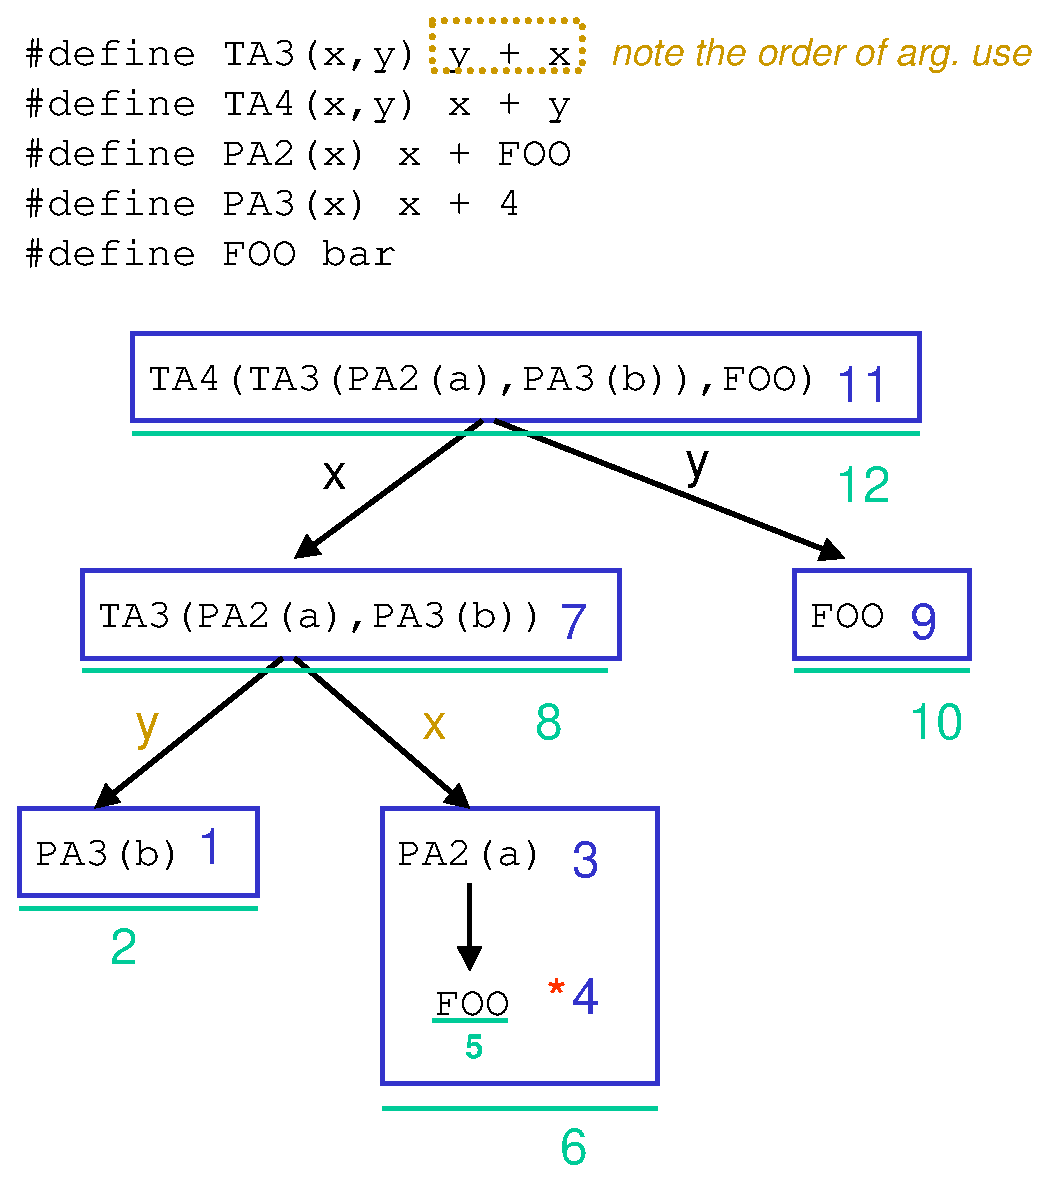
\includegraphics[width=0.45\linewidth]{figs/tree-expn.eps}
    \caption{Post-order traversal of an example macro expansion and the
      hooks that are called. Blue numbers are \texttt{EXPAND\_MACRO}
      actions, green numbers are \texttt{MACRO\_CLEANUP} actions; \eg{}
      the fifth hook \pcp{} invokes is \texttt{MACRO\_CLEANUP} for
      ``\texttt{FOO}''.  The ``cleanup'' means that the macro has been
      fully expanded and is ready to be substituted into the output text
      (or parsed by \pcp{}). Note that between actions 11 and 12, numerous
      \texttt{TOKEN} actions occur.  In general, the tree need not be
      binary, but note that the leaves of a node are the arguments in
      the order of appearance in that node's macro expansion (not their
      order in the list of formal parameters).}
    \label{fig:tree-expn}
  \end{center}
\end{figure}

\begin{figure}[p]
  \begin{center}
    \leavevmode
    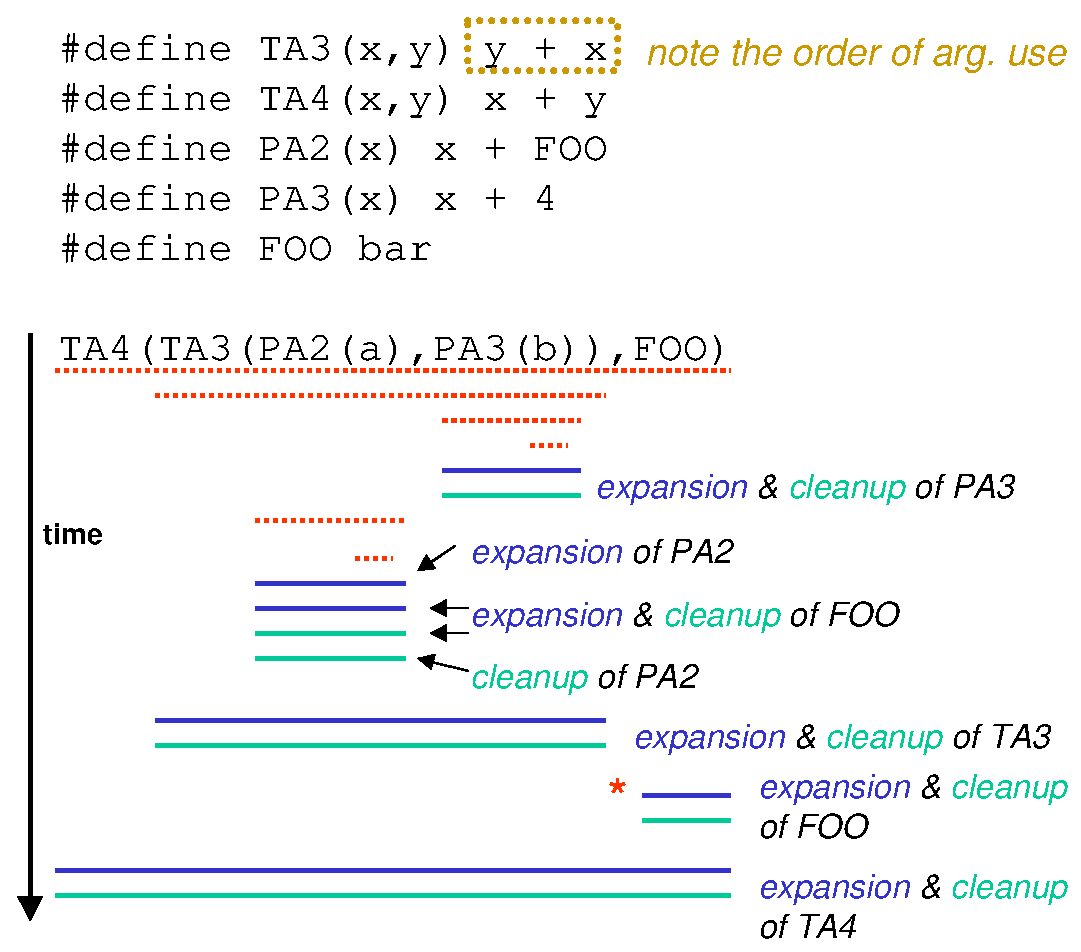
\includegraphics[width=0.45\linewidth]{figs/text-expn.eps}
    \caption{Another view of an example macro expansion and the hooks
    that are called.  Red dotted lines are the nestings of macro
    expansions as the algorithm recurses.  Blue lines are
    \texttt{EXPAND\_MACRO} actions on the underlined macro invocation,
    green lines are \texttt{MACRO\_CLEANUP}.}
    \label{fig:text-expn}
  \end{center}
\end{figure}

Consider the example illustrated in figures \ref{fig:tree-expn} and
\ref{fig:text-expn}.  When the \texttt{MACRO\_EXPAND} hook is called for
\texttt{FOO} (marked with a asterisk star in the figures), we have:

\begin{verbatim}
   @nests                   == ( TA3#1; TA4#1 )
   MacroExpansionHistory()  == ( PA2#Body )
\end{verbatim}

\noindent The \texttt{@nests} list tells us we are expanding the first
argument of macro \texttt{TA3}, which itself was the first argument of
macro \texttt{TA4}.  The \texttt{MacroExpansionHistory()} backcall
provides the remaining information about this expansion: that the
expansion came from the body of the earlier expansion of macro
\texttt{PA2}.  From figure~\ref{fig:text-expn}, the \texttt{@nests} list
for a given expansion corresponds to the sequence of red dotted lines
directly above and completely overlapping the blue line representing
that expansion.  Similarly, the \texttt{MacroExpansionHistory()}
backcall's returned list can be visualized as the stack of blue expansion
lines directly above the expansion in question (those that have not
already been paired with a green line representing the completion of
their expansion).

%% Emacs support
\subsection{Program understanding support in Emacs}
%advantage over font-lock mode that you get information from the actual
%parse, not by some lexical rules which may cause a mismatch
Some of the analyses \pcp{} supports generate excessive amounts of
information that is not easy to comprehend in raw form.  For example,
the mapping between unprocessed source code and preprocessed code aids
program understanding little when existing only in a data structure in a
\Perl{} script.  The standard module of hook utilities provides a
mechanism to output character-indexed annotations of the source code.
These annotations are Emacs Lisp source code which manipulate Emacs text
properties of character ranges when evaluated~\cite{GNUELisp}.  This provides a useful
(indeed, essential during debugging) mechanism for visualizing the
results of the analyses within the context of the code analyzed.  As the
cursor is moved over source code that has been annotated, a subsidiary
Emacs frame dynamically displays the annotations applicable to the
user's current location. See figure~\ref{fig:emacsdocprop} for an
example.

\begin{figure}[p]
  \begin{center}
    \leavevmode
    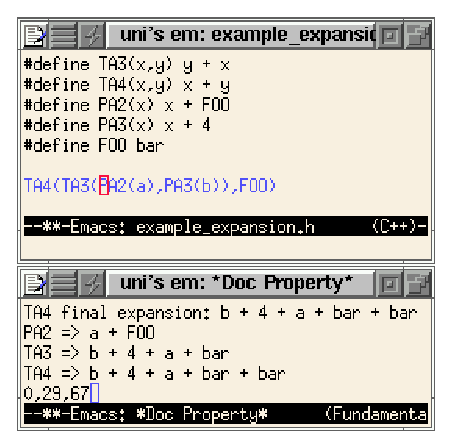
\includegraphics{figs/doc-prop.ps}
    \caption{A view of Emacs using the author's ``doc-property-display''
      feature to dynamically view textual annotations of results of the
      analyses of \pcp{}.  The red outline box in the top frame
      corresponds to the user's cursor, and the lower frame lists the
      various text properties attached to the character under the
      cursor.  The bottom frame potentially changes after each cursor movement.}
    \label{fig:emacsdocprop}
  \end{center}
\end{figure}


Annotating text makes more sense than annotating the abstract syntax
tree for several reasons.  First, \Cpp{} operates at a textual level.
As we have seen, the unprocessed source code cannot necessarily be
viewed as an ordinary abstract syntax tree.  Even if a generalized tree
could be constructed, no available environment provides adequate means
of interacting with the large, complicated trees that inevitably result
from realistic packages.~\footnote{The intentional programming group at
  Microsoft Research is actively investigating this
  area~\cite{MSIPPersonal}.}  Additionally, text permits using Emacs as the
target interaction environment. This allows software engineers to
augment Emacs's other powerful source code understanding tools (\eg{}
\texttt{font-lock-mode}, \texttt{etags}, \texttt{OOBrowser}, \etc{}.)
with their own annotations supplied by \pcp{} analyses.

%% Better than AST for representing the source because cpp is textual
%% Also ASTs not ready for prime-time use

\subsection{Interactions among components}

Given a straightforward preprocessor and parser front end, some analyses
are impossible.  For example, since the preprocessor will skip code as
instructed by conditional compilation directives, that source will never
be seen by the parser, leaving certain questions unanswered.  The
\texttt{doxifdef()} and \texttt{doif()} backcalls provide the code that is
skipped as an argument, but only as literal text.  For an analysis to
reason about the whole source program (not just one configuration), the
skipped code must be exposed to the parser as if it were not removed by
the preprocessor.

The general mechanism for inserting arbitrary source text for the parser
to handle is the \texttt{PushBuffer()} backcall.  Since such program text
can include arbitrary preprocessor directives and \C{} code, we must
ensure that the state of neither the preprocessor nor the parser is
permanently changed after the ``for analysis only'' parsing of the
skipped code.  The data structures that must be preserved are the
preprocessor's hash table of macros and the parser's current stack of
states and symbol table.  The backcalls \texttt{PushHashTab()} and
\texttt{PopHashTab()} save and restore the preprocessor's table of
definitions so that preprocessor directives in skipped code will not
affect \Cpp{} when normal processing resumes.  For the parser, the
backcalls \texttt{EnterScope()} and \texttt{ExitScope()} provide similar
functionality.  Additionally, \texttt{YYPushStackState()} and
\texttt{YYPopStackState()} save and restore the stack of parser states.

Numerous other backcalls provide additional support for querying and
interacting with the parser.  \texttt{ParseStateStack()} returns the
list of states in the parsers stack; this exposes information about
what constructs might be legal (for example, determining whether
declarations may be permitted).  \texttt{SetStateStack()} permits
explicitly changing the parser's stack of states, perhaps to reset to a
top level construct or attempt to reparse text using a different start
state of the parser.  Using \texttt{YYFCompareTopStackState}, an
analysis can easily check whether the ``if'' block and the ``else''
block of an \ppd{ifdef} directive leave the parser in the same state;
a warning could identify instances where this probably desirable
property is violated.

% PushBuffer

% ParseStateStack
%% lets you know where you're at (in an array size specifier; is a decl
%% allowable here?)
% SetParseStateStack

% YYPopAndRestoreStackState
% YYPushStackState
% YYSwapStackState
% YYPushDupTopStackState
% YYFCompareTopStackState

% Permits using the parser to parse individual pieces of code you're
% interested in

\subsection{Performance}

Although no tuning has been done yet, \pcp{} exhibits excellent
performance comparable to an optimizing compiler.  For \texttt{gcc} to
compile and optimize the 5,000 lines of the \texttt{bc} package (an
arbitrary precision arithmetic language interpreter) required 38 seconds
on the author's Pentium Pro 200 Linux machine. Running \pcp{} with its
test script consisting of 600 lines of hooks testing and writing debug
output for every event took 4 minutes.  Remove hooks for
\texttt{CPP\_OUT} and \texttt{TOKEN} (the most frequently invoked hooks)
reduced the running time to 50 seconds.  With all action code turned
off, the running time was reduced by a factor of 5, requiring less than
10 seconds.  Using the \texttt{--noparse} option hardly reduced the
running time at all.

\section{Automating replacement of \ppd{define}s with constants}
\label{sec:xform}

%% Transformations really about understanding
Transforming code is mostly about analysis.  To safely replace a \Cpp{}
construct with a language feature, we must be sure that doing so does
not break the existing code;  semantics and performance should be
preserved or improved.  Compilers necessarily sit at one extreme of the
transformation spectrum---they must absolutely preserve semantics of
their source language as they lower the level of abstraction to machine
instructions.  

Software engineering source-to-source transformations can afford to be
slightly less stringent.  \pcp{} attempts to provide an analysis
framework powerful enough to be as accurate as a compiler, while
requiring minimal programming effort to perform the analysis.  The
standard module of action hooks focusses on assisting a knowledgeable
user understand the code and locate areas which might cause difficulty.
Nothing inherent to the framework disallows completely automatic
conversions of entire packages, but while the analyses and
transformations are still being refined, an interactive editing-based
approach is preferable.

A fairly simple transformation that is well within \pcp{}'s capabilities
is replacing \ppd{define}s of constant symbols with language-proper
constant variables.  Though the transformation sounds trivial, there are
several subtleties.  Consider the example in
figure~\ref{fig:def_example}.  Each of \texttt{FOO}, \texttt{FUD},
\texttt{BAR}, \texttt{BAZ}, \texttt{BING}, and \texttt{BONG} expand to
integers, and so are candidates for replacement with \C{} \texttt{const
  int}s.

\begin{figure}[hbt]
\begin{center}
\begin{small}
\begin{pseudocode}[5.5in]
#include <stdio.h>

#ifdef CCD1
#  define FOO 1
#endif
#ifdef CCD2
#  define FOO 2
#endif

#define FUD 3
#define BAR 4
#define BAZ 5
#define BING 6

int
main(char **argv, int argc)
{
  int fud = FUD;
  int BONG = -1;
  int rgi[BING];
  printf("%d, %d, %d, %d, %d, %d\n",FOO,FUD,BAR,BAZ,BING,BONG);
#define BAR -2
#define BONG 7
  printf("%d, %d, %d, %d, %d, %d\n",FOO,FUD,BAR,BAZ,BING,BONG);
  return 0;
}

#undef FUD
\end{pseudocode}
\end{small}
\caption{Example illustrating some subtleties when converting \ppd{define}s
  into constant declarations.}
\label{fig:def_example}
\end{center}
\end{figure}

However, upon closer examination, there are several reasons why we
conservatively should not simply replace the definitions with
corresponding static variable declarations:

\begin{itemize}
\item \texttt{FOO} has two definitions that are not necessarily mutually
      exclusive (they would have to be to ensure that the program would
      not produce \Cpp{} warnings).
\item \texttt{BAR} is redefined (this definitely produces a \Cpp{}
      warning).  Additionally, the location of the second definition is
      inappropriate for a \C{} declaration (this is irrelevant if we
      really are converting to \CPP{}).
\item \texttt{BING} is used as an array bounds specifier in the
      declaration of \texttt{rgi}.  Array bounds specifiers are required
      to be ``constant expressions'', which ANSI \C{} does not consider
      a \texttt{const int} to be.  \texttt{gcc} and \CPP{} both do allow
      this form.\footnote{Though only recently did the \CPP{} draft standard
      evolve to handle this form properly inside of a class
      declaration~\cite{CD2DraftStandard}.  Because of the
      ``misfeature'' of such declarations still requiring definitions
      outside of the class, Stroustrup still recommends using
      \texttt{enum}s for static integral constant members (\ie{} the
      ``enum hack'')~\cite[p.~249]{Stroustrup97}.}
\item \texttt{BONG} is used as a variable identifier before later being
      defined.  Note that the \ppd{define} of \texttt{BONG}, like that
      of \texttt{BAR}, is at an inappropriate location for a \C{}
      declaration.  Converting to a declaration and moving forward in
      the code would result in a name conflict with the integer variable
      \texttt{BONG}\footnote{Situations like these are why the naming
      convention that macro names are all uppercase proves useful.}
\end{itemize}

\noindent Using \pcp{} with its standard actions, all of the above
situations are recognized.  The source code gets annotated so that when
the user's cursor is resting on a definition, Emacs presents the
warnings and other messages related to that definition.  Also tracked
are the definition and uses chains of the macro names.  Thus, when the
software engineer would like to perform the suggested transformation, a
single Emacs command makes the necessary changes.  \pcp{} will suggest
using a \texttt{static const int} variable if there are no uses in
array-bounds specifiers, otherwise it will suggest using an anonymous
\texttt{enum} declaration (which is an ANSI \C{} constant expression).

Converting a \ppd{define} into a variable or \texttt{enum} declaration
is not usually sufficient.  Reusing a previous macro name will generally
violate the naming convention that only macro names are all
uppercase. If there are no name conflicts, \pcp{} will recommend
a more appropriate name for the real-variable version of the old
\ppd{define}d constant.  For example, \texttt{BING} will be renamed
\texttt{bing}, and all the uses will be updated.  Note, though, that
replacing \texttt{FUD} with \texttt{fud} will result in a name conflict
not unlike the problem with \texttt{BONG}, above.  In such instances,
the problem is annotated, and the change is made to the \ppd{define}
without the corresponding name change.

Because all of the heuristics for the transformation are implemented in
\Perl{} action code, they are easy to develop, test, and refine.  Other
simple analyses \pcp{} currently performs include syntax-highlighting of
the source code, call graph extraction, and the previously-mentioned
macro expansion tracking on both the unprocessed source code (what it
expands to) and on the preprocessed output code (where it expanded
from).

\section{Related Work}
\label{sec:related}
Numerous tools exist for assisting the software engineer in
understanding and manipulating her source code.  Griswold and Atkinson
review a number of them while motivating their \texttt{TAWK} tool~\cite{Griswold96}.
\texttt{TAWK} uses \C{} as its action language and matches patterns in
the abstract syntax tree.  They take significant pains to handle macros
correctly, since they use a parser which could otherwise be too
fragile.  They try to parse each macro definition as an expression,
allowing macro arguments to be types, as well.  If that succeeds, the
macro is left unexpanded in the code and becomes a node resembling a
function call in their AST.  About 92\% of macro definitions in the two packages
they studied parsed acceptably.  For the remaining 8\%, they expanded
uses before feeding the resulting tokens to their parser.  Griswold and
Atkinson note that counting macro expansions is difficult, yet this is
something \pcp{} does with ease.

The ``Intentional Programming'' group at Microsoft Research, headed by
Charles Simonyi, is interested in preserving preprocessor abstractions
as they import legacy \C{} code into their system.  Rammoorthy
Sridharan, a researcher in the group, developed a technique for handling
preprocessor directives by expanding everything while marking each token
with its textual derivation by the preprocessor.  Before preprocessing,
conditional compilation directives are converted to stylized variable
declarations. These declarations and the other source is then run
through a \CPP{} parser to create an AST.  The annotations decorate the
abstract syntax tree, and ``enzymes'' privy to the meaning of the
stylized variables process the tree in an attempt to identify
abstractions.  When macro expansions vary from use to use (\eg{}
\texttt{\_\_LINE\_\_}, the variable text is added as an extra argument
to the macro, and the different values are explicitly passed at the call
sites. Especially unusual uses of conditional compilation directives
cause problems because of constraints on where \CPP{} declarations may
go, but generally the group is optimistic about the possibilities of
their approach~\cite{MSIPPersonal}.

LCLint attempts to analyze macro definitions for
dangerous or error-prone constructs.  It allows, for example, to
annotate that a macro argument needs to be side-effect free at an
invocation site, and can generate a warning message if this constraint
is violated.  Evans's focus is on finding errors, and the
analysis on macro expansions is fairly uninvolved
~\cite[Ch.~8]{LCLint}.

Cordy and Carmichael designed \texttt{TXL} as a language to support
arbitrary transformations on abstract syntax trees~\cite{TXL}.  Their
work is not targeted specifically to \C{} code, and ignores issues
relating to the preprocessor.  Their tool uses a grammar to parse the
language and creates the tree, then applies some tree transformations
directly on the tree, and uses an ``unparser'' to write the new source
code back.  Their transformations are similar to the ``syntax macros''
suggested for use with \C{} by Weise and Crew~\cite{Weise93}.  These
constructs resemble the macros provided by Lisp~\cite{Steele90}, and
have the nice feature of syntactic safety, guaranteeing that macros can
not introduce syntax errors. Crew also created \texttt{ASTLOG}, a
\textsf{Prolog}-inspired language for examining abstract syntax trees.
Again, he largely ignores the preprocessor, instead assuming a parse
tree as the initial representation.

Stroustrup explains that making the preprocessor redundant was a design
goal of \CPP{}.\footnote{Stroustrup also discusses differences between
  \C{} and \CPP{} which could cause other problems when re-targeting
  legacy \C{} code to a \CPP{}
  compiler~\cite[p.~816-820]{Stroustrup97}.} Though \CPP{} provides no
feature to replace the obviously still-needed \ppd{include} directive,
Stroustrup discuss the form that construct
might take.   Carroll and Ellis make the strong claim that ``C++ provides
mechanisms that obviate the need for most
macros''~\cite[p.~147]{Carroll95}.  They list numerous uses of the
preprocessor and describe the \CPP{} language features that could
replace them.  Their advice is mostly prescriptive and is directed to
the new \CPP{} programmer who might be inclined to overuse \Cpp{}
constructs as a crutch instead of exploiting \CPP{} language features.
They do not directly address converting existing use of \Cpp{} in legacy
code.  Reiss and Davis casually mention a research project that helps
the user restructure programs by ``translat[ing] an existing \C{}
program into \CPP{}''~\cite[p.~2]{Reiss90}, but nothing further is
mentioned about the project.\footnote{Personal inquiries of that paper's
  authors also led to no pointers.}

Siff and Reps also consider a transformation of \C{} code to \CPP{}.
They use type inference to generalize \C{} functions and create a
reusable template-based \CPP{} function.  Their technique applies only
to  \C{} functions after they have been preprocessed.

Davis provides a thorough review of the issues involved in translating
\CPP{} language constructs to Java.  He ignores the preprocessor and its
contribution to \CPP{} source code artifacts~\cite{Davis97}.  Laffra's
\texttt{C2J} and Tilevich's derived \texttt{C2J++} claim to convert \C{} and
\CPP{} to Java code.  Their approach is a combination of lexical and
parser-based, and is focussed only on reducing the tedious editing when
porting an application to Java.  They use \Cpp{} to preprocess, and
claim to only convert about 85\% of the code correctly.

Krone and Snelting analyze conditional compilation directives in the
context of a lattice-theoretic framework for inferring configuration
(versioning) structures from the source code.  They study how \ppd{if}
guards depend on and relate to each other, and provide a means of
visualizing the relationships with the goal of improving the
programmer's understanding of the structure and properties of the
configurations~\cite{Krone94}.

% Summary & Future work
\section{Summary and Future Work}
\label{sec:summary}


% Framework problems
%** Fairly dependent on internals of the preprocessing and parsing peculiarities of the tools
%** Huge effort in making the hooks interface complete; existing hooks motivated by need not by design
%** Also data structure sharing; duplication of work between perl code and cpp/parser structures
%** AST going to waste for now; ast viewing w/ Tk?

% Possible applications
%** Syntax highlighting
%** Source + output annotations
%** Tags generation
%** Call graph extraction (add summaries to fns)
%** parser debugging, teaching
%** multi-version reasoning

%* Convert to Java
%* C++ parser; C++ code still uses preprocessor too much
%* Multiple translation units: use technique like CIA++ ~\cite{CIA++90}

%* Use configuration structures to bound the number of cpp tables and
%scope table variants required

\appendix
\newpage

%%FIXGJB: order and organize these
\section{Action hooks called by \pcp}
\begin{footnotesize}
\label{sec:hooks}
\begin{itemize}
\sloppy
\hook{STARTUP}{} Called immediately after the perl parser is initialized.
\hook{STARTPARSE}{} Called just before the bison parser is started (i.e., before yyparse()).
\hook{EXIT}{\$return\_\-exit\_\-code} Called just before the system exit() call.
\hook{HANDLE\_\-DIRECTIVE}{\$directive\_\-name} Called exactly once for each directive.  \$directive\_\-name is
the directive as it appeared in the source code with the leading \pphash{} removed.
\hook{DO\_\-DEFINE}{\$s\_\-start, \$s\_\-end, \$name\_\-args\_\-body} Called exactly once for each \pphash{}define. 
Arguments give the source code character offsets of the line and the 
unprocessed rest of the line including the name of the macro, its arguments
and its definition.
\hook{PRE\_\-DO\_\-UNDEF}{\$s\_\-start, \$s\_\-end, \$mname} Called exactly once for each \pphash{}undef.
Arguments give the source code character offsets of the line and the
name of the macro being undefined.  This hook is called just before
the macro is undefined, so its definition still exists 
in the preprocessor's state.
\hook{DO\_\-UNDEF}{\$s\_\-start, \$s\_\-end, \$mname} Called exactly once for each \pphash{}undef.
Arguments give the source code character offsets of the line and the
name of the macro being undefined.  This hook is called immediately after
the macro is undefined.
\hook{DO\_\-INCLUDE}{\$s\_\-start, \$s\_\-end, \$filename\_\-given, \$filename\_\-resolved, \$flags} 
Called exactly once for each \pphash{}include,
\pphash{}include\_\-next, or \pphash{}import directive.  Source coded character offsets of
the line are given. Also, \$filename\_\-given is the name of the
file to be included as written in the source;  \$filename\_\-resolved is the
fully qualified path name of the file to be read; and  \$flags is a bitmap
with three relevant masks:  \$ANGLE\_\-BRACKETS, for whether the filename appeared
in angle brackets signifying a system include file; \$SKIP\_\-DIRS, for whether this
is an \pphash{}include\_\-next directive; and \$IMPORTING, for whether this is an \pphash{}import
directive.
\hook{DO\_\-IF}{\$s\_\-start, \$s\_\-end, \$conditional, \$skipped, \$value} 
Called exactly once for each \pphash{}if 
(not \pphash{}ifdef or \pphash{}ifndef) directive seen by the preprocessor. In particular,
note that normally, nested \pphash{}ifXX-s that are ignored will not invoke this hook.
Arguments give the source code character
offsets of the directive; \$conditional is the guard checked, \$skipped is
the literal text that is skipped (conditional was false if this is non-empty), and
\$value is 1 iff the \$conditional evaluated to true (defined), 0 otherwise.
\hook{DO\_\-XIFDEF}{\$s\_\-start, \$s\_\-end, \$kind, \$conditional, \$trailing\_\-garbage, \$skipped, \$fSkipping, \$s\_\-branch\_\-start}
Called exactly once for each \pphash{}ifdef or \pphash{}ifndef.
The arguments are the same as for the DO\_\-IFDEF hook, except \$kind is either
"IFDEF" or "IFNDEF" depending on the type of conditional; \$fSkipping
replaces the \$value argument and is non-zero iff the conditional fails
(i.e., an IFDEF with a not-defined macro, or an IFNDEF with a defined macro);
\$s\_\-branch\_\-start gives the source code character offset of the start of
the branch taken.  Note that this hook is called after the DO\_\-IFDEF or DO\_\-IFNDEF
hook.
\hook{DO\_\-IFDEF}{\$s\_\-start, \$s\_\-end, \$conditional, \$trailer, \$skipped, \$value}
Called exactly once for each \pphash{}ifdef
(not \pphash{}if or \pphash{}ifndef) directive seen by the preprocessor. In particular,
note that normally, nested \pphash{}ifXX-s that are ignored will not invoke this hook.
Arguments give the source code character
offsets of the directive; \$conditional is the name checked for defined-ness;
\$trailer is whatever follows that name on the same line (usually empty); \$skipped is
the literal text that is skipped (conditional was false if this is non-empty), and
\$value is 1 iff the name from the \$conditional was defined, 0 otherwise.
\hook{DO\_\-IFNDEF}{\$s\_\-start, \$s\_\-end, \$conditional, \$trailer, \$skipped, \$value}
Called exactly once for each \pphash{}ifndef
(not \pphash{}if or \pphash{}ifdef) directive seen by the preprocessor. In particular,
note that normally, nested \pphash{}ifXX-s that are ignored will not invoke this hook.
Arguments give the source code character
offsets of the directive; \$conditional is the name checked for defined-ness;
\$trailer is whatever follows that name on the same line (usually empty); \$skipped is
the literal text that is skipped (conditional was false if this is non-empty), and
\$value is 1 iff the name from the \$conditional was not defined, 0 otherwise.
\hook{DO\_\-ELSE}{\$s\_\-start, \$s\_\-end, \$orig\_\-conditional, \$trailer, \$skipped, \$fSkipping, \$s\_\-start\_\-branch}
Called exactly once for each \pphash{}else directive seen by the preprocessor. In particular,
note that if the directive is skipped due to another outer conditional, this
hook does not get called.
Arguments give the source code character
offsets of the directive; \$orig\_\-conditional is the guard in the
matching \pphash{}ifXX directive; 
\$trailer is whatever follows \pphash{}else on the same line (usually empty); \$skipped is
the literal text that is skipped (if any); \$fSkipping is 1 iff
this \pphash{}else clause's guarded text got skipped; \$s\_\-start\_\-branch is a souce code
character offset of where the branch begins, if it's used, or the character
following the skipped text if not.
\hook{DO\_\-ELIF}{\$s\_\-start, \$s\_\-end, \$already\_\-did\_\-clause, \$conditional, \$skipped, \$value}
Called exactly once for each \pphash{}elif directive seen by the preprocessor. In particular,
note that if the directive is skipped due to another outer conditional, this
hook does not get called.
Arguments give the source code character
offsets of the directive; \$already\_\-did\_\-clause is 1 iff one of the
earlier \pphash{}ifXX or \pphash{}elif-s succeeded (thus implying the code guarded will be skipped);
\$conditional is the conditional tested; \$skipped is the skipped code (if any);
and \$value is what \$conditional evaluated to.  The code guarded is
included iff !\$conditional and \$value, in which case \$skipped will be empty.
\hook{DO\_\-ENDIF}{\$s\_\-start, \$s\_\-end, \$orig\_\-conditional, \$trailer}
Called exactly once for each \pphash{}endif directive seen by the preprocessor. In particular,
note that if the directive is skipped due to another outer conditional, this
hook does not get called.
Arguments give the source code character
offsets of the directive; \$orig\_\-conditional is the guard of the matching
\pphash{}ifXX directive; \$trailer is the text following the \pphash{}endif (often empty);
\hook{CREATE\_\-PREDEF}{\$mname, \$expansion, \$num\_\-args, \$internal\_\-expansion, \$file, \$line, \$r\_\-argnames, \$flags, \$internal\_\-expansion\_\-args\_\-uses... }
Called once for each predefined macro CPP installs.
\$mname is the name of the macro, \$expansion is its expansion [as literal text], 
\$num\_\-args is the number of arguments it takes, \$internal\_\-expansion is an
internal representation of the expansion (which is interpreted in the 
context of \$internal\_\-expansion\_\-args\_\-uses, see cpplib.c), \$file and \$line
can safely be ignored, \$r\_\-argnames is a comma separated list of the
argument names in reversed order, and \$flags is a bitmask of two flags
\$flags \& \$PREDEFINED is true if this is a predefined macro (always for this hook)
and \$flags \& \$RESTARGS is true if this macro's last argument swallows 
remaining arguments (special gcc cpp feature).
\hook{CREATE\_\-DEF}{\$s\_\-start, \$s\_\-end, \$mname, \$expansion, \$num\_\-args, \$internal\_\-expansion, \$file, \$line, \$r\_\-argnames, \$flags, \$internal\_\-expansion\_\-args\_\-uses... }
Called once for each macro definition read by  CPP.
\$s\_\-start and \$s\_\-end are the source code character offsets of the definition,
\$mname is the name of the macro, \$expansion is its expansion [as literal text], 
\$num\_\-args is the number of arguments it takes, \$internal\_\-expansion is an
internal representation of the expansion (which is interpreted in the 
context of \$internal\_\-expansion\_\-args\_\-uses, see cpplib.c), \$file and \$line
give the filename and line number where the definition occurs, 
\$r\_\-argnames is a comma separated list of the
argument names in reversed order, and \$flags is a bitmask of two flags
\$flags \& \$PREDEFINED is true if this is a predefined macro (never for this hook)
and \$flags \& \$RESTARGS is true if this macro's last argument swallows 
remaining arguments (special gcc cpp feature).
\hook{DELETE\_\-DEF}{\$mname, \$fExists}
Called once for each macro name that is undefined for any reason (this is
a low level hook called when you attempt to remove a macro name from the 
table of macros,
also HI\_\-DO\_\-UNDEF for the high level hook).  \$mname is the name of the
macro, and \$fExists is 1 iff that macro name used to be defined.
\hook{SPECIAL\_\-SYMBOL}{\$symbol, \$enum\_\-node\_\-type}
Called once for each special symbol (e.g., \_\-\_\-FILE\_\-\_\-) that gets expanded.
\$symbol is the literal text of the symbol, \$enum\_\-node\_\-type is an index
into @enum\_\-node\_\-type giving the C constant corresponding to that symbol
(usually better to just use \$symbol instead).
\hook{EXPAND\_\-MACRO}{\$s\_\-start, \$s\_\-end, \$mname, \$expansion, \$length, \$raw\_\-call, \$has\_\-escapes, \$cbuffersDeep, \$cnested, @nests, \$cargs, @args}
Called once for each macro expansion in C source (i.e., not for expansions
in \pphash{}ifXX guards). \$s\_\-start and \$s\_\-end are the source code character offsets
of the macro invocation; \$mname is name of the macro, \$expansion is what
replaces \$mname in the text (subject to further expansion, of course); \$length
is the number of characters in that expansion, \$raw\_\-call is how the call
appeared in the source (includes the macro name), \$has\_\-escapes is 0 if the
source buffer is actual source text (i.e., if this is a top level expansion),
otherwise it is a 1 (escapes has marked with @- preceding the macro name);
\$cbuffersDeep is how many levels of expansion the text
has undergone beyond the source text (0 means the macro occurrence appeared
directly in the source code); \$cnested tells how many elements are in @nests
(so you can separate its arguments from @args); @nests is non-empty when this
expansion is an argument to another macro---see the body of the paper for 
a complete explanation.
\$cargs tells how many arguments \$mname takes; and @args contains argument
expansion and use information.  Each argument contributes 7 elements to @args
plus a pair of elements for each use;  e.g., if the first argument was used 3 times
it would have 7 + 3*2 = 13 elements in @args describing its expansion.  The
first 6 arguments are \$raw,\$r\_\-offset,\$expanded,\$e\_\-offset,\$stringified,\$s\_\-offset
which correspond to the raw, expanded, and stringified representations of the
argument.  The \$X\_\-offset elements are internal offsets into a token buffer
and can usually be ignored.  \$stringified may be empty if the argument was
never stringified during the macro expansion.  The seventh element for each
argument tells how many times that argument was used in the expansion, and
successive pairs of elements give character offsets to the appearance of those
arguments in the expansion.  For example if argument 1 is used 3 times, there could
be (3, 5,6, 9,11,  14,18) as the final elements of the @args list.  Note that
because the third expansion is longer than the first two (4 characters instead of
just two), it must have been stringified.
\hookobsoleted{MACARG\_\-EXP}{\$mname, \$raw, \$number}
\hook{MACRO\_\-CLEANUP}{\$s\_\-start, \$s\_\-end, \$mname, \$c\_\-nested, @nests}
Called once for each macro expansion buffer as it is removed 
from the stack of text buffers.  \$s\_\-start and \$s\_\-end give the source
code character position offset of the text which expanded into the text
that is in the buffer currently being cleaned and pop-ped;  \$mname is the
name of the macro that resulted in that expansion; \$c\_\-nested and @nests
are obsoleted.  Note that to get the full text of the expansion, you must
track successive strings passed to the CPP\_\-OUT hook, and reset the
string used to accumulate the expansion when the CbuffersBack backcall
is 1 in this hook (meaning you are cleaning up a top level macro expansion).
See cpphook.pm for an example.
\hook{IFDEF\_\-MACRO}{\$s\_\-start, \$s\_\-end, \$mname, \$expansion, \$length, \$raw\_\-call, \$has\_\-escapes, \$cbuffersDeep, \$cnested, @nests, \$cargs, @args}
Called once for each macro expansion in \pphash{}if directives.  The arguments
passed to the hook are the same as those for the EXPAND\_\-MACRO hook, see its
documentation for details.  Note, though, that macros are not usually
expanded in \pphash{}ifdef and \pphash{}ifndef directives, they are simply tested for
defined-ness by lookup in the symbol table, thus triggering the IFDEF\_\-LOOKUP\_\-MACRO
hook, not this one.  A form such as "\pphash{}if FOO" will trigger this hook, however.
\hook{IFDEF\_\-LOOKUP\_\-MACRO}{\$mname, \$f\_\-defined}
Called once for each macro name lookup done during conditional compilation
guard checking.  The arguments are:
\$mname is the macro name being looked up; \$f\_\-defined is non-zero
iff the macro has been defined.  Use backcalls to get the expansion if
it is desired.
\hook{COMMENT}{\$s\_\-start, \$s\_\-end, \$comment\_\-text, \$how\_\-terminated, \$c\_\-lines}
Called once for each comment in the source code seen by preprocessor (i.e.,
comments conditionally-compiiled out will not normally invoke this hook).
\$comment\_\-text is the text of the comment, \$how\_\-term is "*/" for C-style
comments, "nl" for a C++ style comment, or "eof" if the comment
was ended by the end of file.
\$c\_\-lines is the number of lines that the comment spans, including partial lines.
\hook{STRING\_\-CONSTANT}{\$s\_\-start, \$s\_\-end, \$string, \$lines}
Called once for each string in the source code or macro/special symbol expansion.
Note that both stringization and symbols like \_\-\_\-FILE\_\-\_\- will invoke this hook
with their string expansions.
Arguments give the source code character offsets of the string, \$string is
the string, and \$lines is the number of lines (or partial lines) that the
string spans.  \$s\_\-start == \$s\_\-end if the string does not actually appear
in the top level source code (e.g, \_\-\_\-LINE\_\-\_\- or gcc's \_\-\_\-FUNCTION\_\-\_\-).
The source code offsets include the string delimiters, the \$string argument
has them stripped, but has not had backslash sequences replaced.
\hook{CPP\_\-ERROR}{\$nominal\_\-fname, \$line\_\-number, \$message, @extra\_\-args}
Called once each time CPP issues an error.  The hook does not interfere
with normal error handling.  Arguments give the current filename and line
number where the error occurred;  \$message is the string (containing printf
percent-escapes) to be printed, and @extra\_\-args are the values to be 
interpolated into the string.
\hook{CPP\_\-WARN}{\$nominal\_\-fname, \$line\_\-number, \$message, @extra\_\-args}
Called once each time CPP issues a warning.  The hook does not interfere
with normal warning handling.  Arguments give the current filename and line
number where the warning occurred;  \$message is the string (containing printf
percent-escapes) to be printed, and @extra\_\-args are the values to be 
interpolated into the string.
\hook{CPP\_\-PEDWARN}{\$nominal\_\-fname, \$line\_\-number, \$message, @extra\_\-args}
Called once each time CPP issues a pedantic warning.  The hook does not interfere
with normal pedantic warning handling.  Arguments give the current filename and line
number where the pedantic warning occurred;  \$message is the string (containing printf
percent-escapes) to be printed, and @extra\_\-args are the values to be 
interpolated into the string.
\hook{CPP\_\-OUT}{\$string}
Called for each sequence of characters cpp is outputting.  This is the
same text as would go to the output file when using just cpp (as in gcc -E).
Full tokens and/or whitespace are emitted per each call to the hook.
Use the CchOutput() and CchOffset() backcalls for output character offset
and source code character offset, respectively.
\hook{ADD\_\-IMPORT}{\$filename, \$filedes\_\-num}
Called for each filename that is \pphash{}import-ed.  Arguments give that
file name and the number of the file-descriptor that file was opened
on (negative iff the file was not found).
\hook{INCLUDE\_\-FILE}{\$filename, \$system\_\-include}
Called for each file that is \pphash{}include-d (not necessarily for each \pphash{}include
directive; this hook won't be called if the file cannot be found).
Arguments are the filename and \$system\_\-include, which is non-zero if the filename
appears to be a system include file (absolute pathname and in a known
system directory);  it is exactly 2 iff the file is a C-language
system header file for which C++ should assume extern "C".
\hook{DONE\_\-INCLUDE\_\-FILE}{\$filename}
Called upon completion of parsing of an included file.  The filename
that what just finished being parsed is the only argument.
\hook{TOKEN}{\$token, \$raw, \$macro\_\-name, \$arg\_\-num, @history}
Called once for each token CPP reads.  \$token is the type of token,
with a leading CPP\_\-; \$raw is the raw characters which constitute that
token; \$macro\_\-name is the name of the macro that expanded to create this token,
or is empty if the token did not result from macro expansion; \$arg\_\-num is -1
if the token did not come from a macro expansion, 0 if it came from the
body of a macro expansion (i.e., not an argument), or positive and equal
to the argument number that produced the token, if from an substitution
of an argument in a macro expansion; @history is obsoleted, use the
MacroExpansionHistory() backcall instead.  Note that the token "CPP\_\-POP"
means that an expansion buffer has been popped from the stack of expansions,
and is not a real lexical token.  This may be removed from future version
so use the POP\_\-BUFFER hook to handle those events.
\hook{FUNCTION}{\$name, \$fStatic}
Called once after an entire function is parsed.  Arguments
give the name of the newly defined function, and \$fStatic is non-zero
iff the function was declared to be static (i.e. not global).
\hook{FUNC\_\-PROTO}{\$name}
Called once after an function prototype (declaration) is parsed.  Argument
gives the name of the newly defined function.  This hook is not called
for complete function definitions -- see HI\_\-FUNCTION for that hook.
\hook{FUNC\_\-CALL}{\$name}
Called once after each function call is parsed.  Only argument is
the name of the function being called.
\hook{TYPEDEF}{\$name}
Called once after each typedef is parsed.  Argument is the name
of the new type.
\hook{VARDECL}{\$name}
Called once after each variable declaration is parsed.  Argument is the name
of the declared variable.
\hook{ANNOTATE}{} Obsoleted
\hook{POP\_\-BUFFER}{\$cbuffersDeep}
Called once for each buffer that is popped off of the stack of
buffers to be parsed. The only argument is the new (after the pop)
number of non-file buffers
deep the stack is.  In particular, when that number is 0, 
the parser is not parsing a macro expansion any longer.
\hook{POP\_\-PERL\_\-BUFFER}{\$cbuffersDeep}
Called once for each perl-pushed buffer that is popped off of the stack of
buffers to be parsed (i.e., those pushed with the PushBuffer() backcall)
The only argument is the new (after the pop)
number of non-file buffers
deep the stack is.  In particular, when that number is 0, 
the parser is not parsing a macro expansion any longer.

\fussy
\end{itemize}
\end{footnotesize}

\newpage

%%FIXGJB: order and organize these
\section{Subroutines provided by \pcp}
\label{sec:backcalls}
\begin{footnotesize}
\begin{itemize}
\sloppy
\backcall{\$token\_\-type}{SzToken}{\$id}
Returns a string identifying what kind of token \textit{id} (an integer) represents.
\backcallobsoleted{(\$cchOffset,\$cbuffersback)}{SumCchExpansionOffset}{}
Gives the source code character position offset and the number of expansions
deep that we currently are.
\backcall{\$cbuffersback}{CbuffersBack}{}
Return the number of macro expansions deep that we currently are in
the current expansion.  This returns 0 if we are not expanding a macro.
The number returned is the number of non-file buffers in the current
stack of expansions (so it is not increased by nested \pphash{}include-s).
\backcall{@expanded\_\-macros\_\-list}{MacroExpansionHistory}{}
Returns a list of strings of the form 
\textit{macro\_\-name}\pphash{}\textit{arg\_\-num}[\textit{cchOffsetEnd}]. 
Each string explains the contents of a current expansion buffer,
and the first string is the top of the expansion stack.
For example, if there is a single item in the returned list
which is the string "MAX\pphash{}1[3]", this means that the current
token came from the expansion of macro MAX and was the first argument
to that macro, ending at character offset 3.  Multiple items
in the returned list mean that a macro expanded to some other
macro which was subsequently expanded.  Argument number 0 signifies
that the token came from the literal body of the macro.
\backcallobsoleted{\$index\_\-of\_\-argument}{ArgOf}{}
Returns the number of the argument from which the current token came.
Prefer using the \$argno parameter passed to the TOKEN hook.
\backcall{\$cch\_\-source\_\-offset}{CchOffset}{}
Returns the character position offset into the current source file.
Use Fname() to get the source file name.
\backcall{\$filename}{InFname}{}
Returns a string giving the name of the main input file (the one
that appeared on the command line.
\backcall{\$filename}{Fname}{}
Returns a string giving the name of the current input file.  This
tracks include-d files and, combined with CchOffset, gives a
unique location in the package.  "@NONE@" returned if no current file.
\backcall{\$filename}{FnameNominal}{}
Returns a string giving the filename corresponding to the current
buffer.  This will be "@NOFILE@" if there is no such file (as is
the case when reading tokens from a macro expansion).
Otherwise it will correspond to Fname().
\backcall{\$encoded\_\-expansion}{ExpansionLookup}{\$macro\_\-name}
Returns the internally-encoded (cpplib-specific) expansion of
the macro with name \texttt{\$macro\_\-name}.  Note that this the string
returned is delimited on either end by "@ " and omits argument occurrences.
"@NOTFOUND@" is return if there is no current macro of the given name.
\backcall{\$cchOutput}{CchOutput}{}
Returns the number of characters already output.  Only non-zero when 
--noparse option is given.
\backcallobsoleted{\$cchCppRead}{CchCppRead}{}
Returns the number of characters that have been read from the
input files.  Prefer using the offsets passed in the various hooks.
\backcall{\$fExpandingMacros}{FExpandingMacros}{}
Returns TRUE iff macros are currently being expanded.
Returns FALSE otherwise.  As arguments are read, macros are not expanded,
and this will return FALSE.
\backcall{@parse\_\-state\_\-list}{ParseStateStack}{}
Returns the current stack of parse state numbers.  The first element is
the top state on the stack.  See the gram.output
file for a listing of what the numbers correspond to.
\backcall{}{SetParseStateStack}{@parse\_\-state\_\-list}
Resets the current stack of parse states so that it is @parse\_\-state\_\-list.
This has the potential to break the parse, and often will outside
of the trivial case of setting the stack of states to what it already is.
\backcall{}{PushBuffer}{\$source\_\-code\_\-string, \$s\_\-start}
Adds \$source\_\-code\_\-string to the being-processed text 
as if it existed in the input at the
current location in the current file. \$s\_\-start tells
where the code to be processed is in the current source
file, or is negative if it does not exist there.
\backcall{}{EnterScope}{}
Enters a new scoping level; useful in combination
with PushBuffer() for causing code to be parsed without
affecting the current symbol table directly.
\backcall{}{ExitScope}{}
Exits the current scoping level; useful in combination
with PushBuffer() for causing code to be parsed without
affecting the current symbol table directly.
\backcall{}{PushHashTab}{}
Copies the current cpp hash table and begins using the copy;  the copy
can later be thrown out using PopHashTab()
\backcall{}{PopHashTab}{}
Throw out a previously pushed cpp hash table; revert to the prior
hash table
\backcall{}{SetParseDebugging}{}
Set the yydebug flag to TRUE for the underlying parser.
This results in extra state change information being sent to stderr.
It has no affect if --noparse is used.  Initially, parser debugging is off.
\backcall{}{ResetParseDebugging}{}
Reset the yydebug flag to FALSE for the underlying parser.  
This terminates sending extra state change information to stderr.
It has no affect if --noparse is used.
\backcall{}{YYPushStackState}{}
Save the entire current state of the parse stack onto a meta stack.
\backcall{}{YYPopAndRestoreStackState}{}
Restore the entire current state of the parse stack from the meta stack.
\backcall{}{YYPopAndRestoreStackState}{}
Throws out the top state stack from the meta stack.
\backcall{}{YYSwapStackState}{}
Switch the current stack state and the one on the top of the meta stack.
\backcall{}{YYPushDupTopStackState}{}
Push another copy of the top element of the meta stack of stack states onto
the meta stack.
\backcall{\$fStacksEqual}{YYFCompareTopStackState}{}
Return TRUE iff the top of the meta stack of state stacks is
identical to the current state stack. Return FALSE otherwise.
\backcall{\$fDefined}{FLookupSymbol}{\$symbol\_\-id}
Return TRUE iff \$symbol\_\-id is found in the current scope.
Return FALSE otherwise.

\fussy
\end{itemize}
\end{footnotesize}

% References
\newpage

\nocite{ARM}
\nocite{Dragon}
\nocite{Glickstein97} % Writing GNU Emacs Ext.
\nocite{Camel}        % Perl 5
\nocite{Perl}        % Perl 5
\nocite{Levine92}     % Lex & Yacc
\nocite{Harbison91}   % C Ref Man
\nocite{Stroustrup97} % C++, 3rd
\nocite{Stroustrup94} % C++, 2nd
\nocite{Kernighan88}  % C, 2nd
\nocite{Flanagan96}   % Java in a Nutshell
\nocite{EmpCpp}
\nocite{EmpCpp-TR}
\nocite{GCC}
\nocite{CTree}
\nocite{TXL}
\nocite{Cordy92}
\nocite{Bison}
\nocite{Flex}
\nocite{Krone94}
\nocite{Griswold96}
\nocite{Atkinson96}
\nocite{CD2DraftStandard}

\bibliographystyle{alpha}
\bibliography{library,articles,pcp3}

\end{document}

%%% Local Variables: 
%%% mode: latex
%%% TeX-master: t
%%% End: 
% LocalWords:  stringization tex fancybox gjb endif cpplib backcall
% LocalWords:  MacroExpansionHistory
